\documentclass[letterpaper]{article}
\usepackage{natbib,alifeconf}

\title{Report of the Neural Network Training for the project: Assessing Economic Development and Planning Interventions in the Built Environment: The Role of Provincial Policies in Québec and Ontario}
\author{Alphonsus Adu-Bredu$^{1}$ \\
\mbox{}\\
$^1$Tufts University, Medford - Massachusetts \\
alphonsus.adu\_bredu@tufts.edu}


\begin{document}
\maketitle

\begin{abstract}
	The dataset was first split into the 6 categories; "depressing", "lively", "safety", "wealthy", "boring" and "beauty". All the operations reported in this paper were made to the depressing category.
\end{abstract}
\section{Data Preprocessing}
After the categorization,the dataset was cleaned up by removing all datapoints that appeared in both the positive and negative sub-categories. The coordinates for all positive datapoints(images that are depressing) were retrieved. 

\section{Downloading images and training neural network}
For the first batch of training, the first 250 coordinates of both the positive datapoints and their corresponding negative datapoints were retrieved and their corresponding street-view images were downloaded. After the images were downloaded, a convolutional neural network was trained on the positive and negative images. 

In training the convolutional neural network, a method called Transfer Learning was employed. We first downloaded Google's pre-trained inception-v3 model and retrained the last two layers in the network with our 250 images. The training process was first ran for 500 iterations. A graph of the training accuracy over the 500 iterations is in Figure 1.

\begin{figure}[!htb]
	\begin{center}
		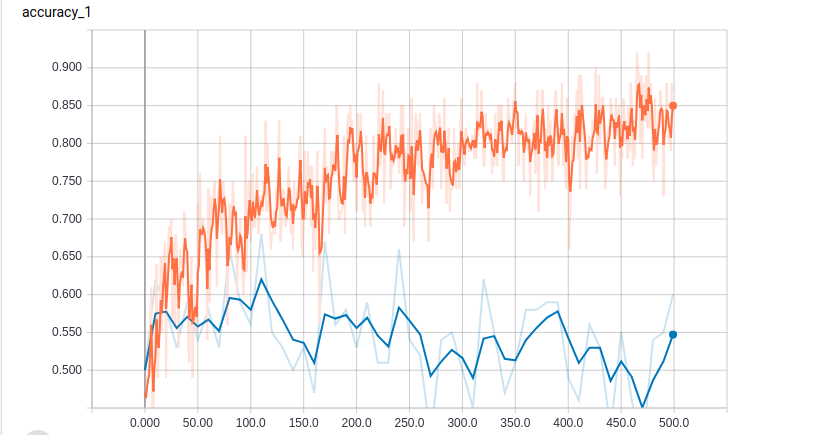
\includegraphics[width=4in]{250_img_500_it_accuracy.png}
		\caption{250 images, 500 iterations. Training accuracy = Red, Cross-validation accuracy=Blue}
		\label{fig1}
	\end{center}
\end{figure}

The average training accuracy was around 85\% while the cross-validation accuracy lingered around 50\%.

The number of iterations was increased to 2500 and the training accuracy rose to 98\% while the cross-validation accuracy still lingered around 50\%. [Figure 2]This meant that our trained model was over-fitting on the training set. A common remedy for this would be to increase the number of training images.\\

\begin{figure}[!htb]
	\begin{center}
		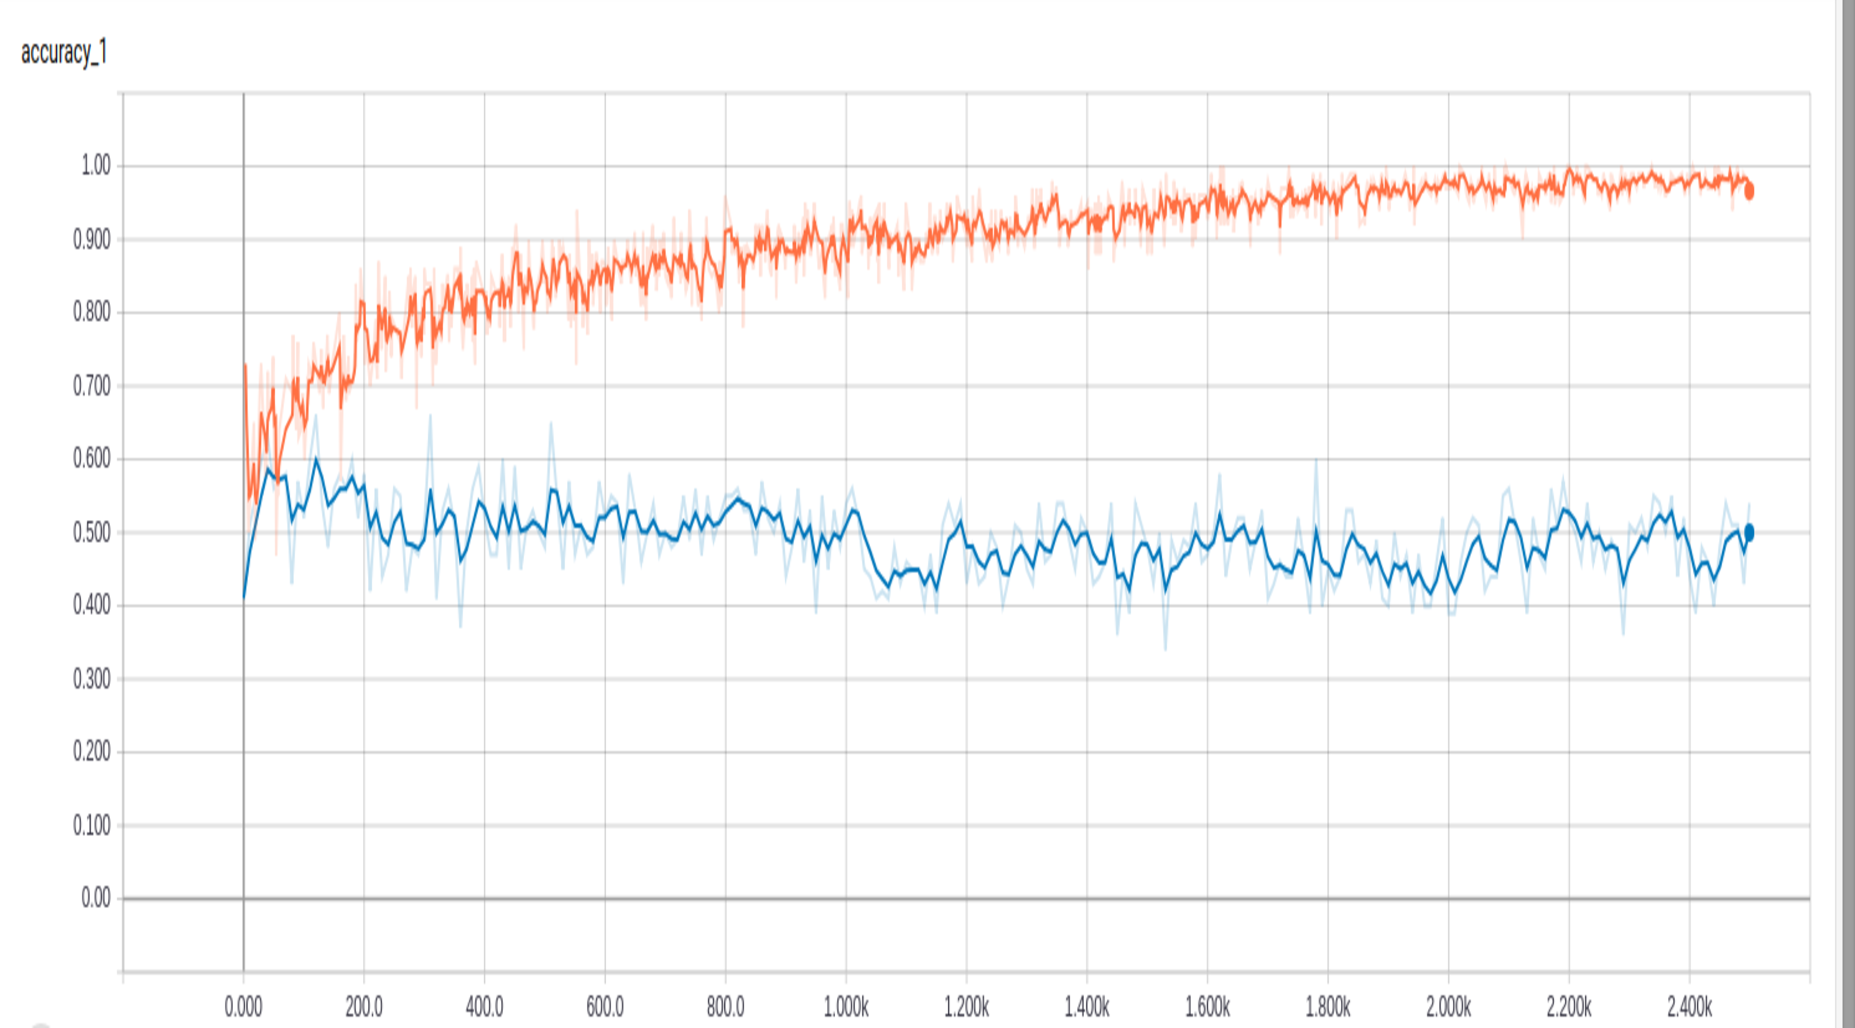
\includegraphics[width=4in]{250_img_2500_it_accuracy.png}
		\caption{250 images, 500 iterations. Training accuracy = Red, Cross-validation accuracy=Blue}
		\label{fig1}
	\end{center}
\end{figure}

\begin{table}[!hbt]
\center{
\begin{tabular}{|c|c|c|}\hline
One & Two & Three\\ \hline\hline
Yes & 0 & 1 \\
Not  & 1 & 0 \\
Maybe & 0.5 & 0.5 \\ \hline
\end{tabular}
}
\vskip 0.25cm
\caption{Sample table caption.}
\end{table}


\footnotesize
\bibliographystyle{apalike}
\bibliography{sample}


\end{document}
